\documentclass[10pt,twocolumn]{article}
\usepackage{hyperref}
\usepackage{courier}
\usepackage{graphicx}
\usepackage{array} % for centering table values with predefined width
\newcolumntype{P}[1]{>{\centering\arraybackslash}p{#1}}
\newcolumntype{M}[1]{>{\centering\arraybackslash}m{#1}}

\title{
	\usefont{OT1}{bch}{b}{n}
	\normalfont \normalsize \textsc{Technology Report} \\ [10pt]
	\huge{
		An R Shiny application for introducing multivariate calibration to
		advanced undergraduate students
	}
}

\author{
	Tom\'as M. Antonelli
	\footnote{E-mail: atmunr@gmail.com},
	Alejandro C. Olivieri
	\footnote{E-mail: oliveri@iquir-conicet.gov.ar}
	\\ \\
	Departamento de Qu\'imica Anal\'itica, Facultad de Ciencias \\
	Bioqu\'imicas y Farmac\'euticas, Universidad Nacional de Rosario, \\
	Instituto de Qu\'imica de Rosario (IQUIR-CONICET), \\
	Suipacha 531, Rosario S2002LRK, Argentina
}

\date{}

\begin{document}

\maketitle

\begin{abstract} During a short chemometrics course in the seventh semester of
the chemistry undergraduate program, students receive a brief theoretical
introduction to multivariate calibration, focused on partial least-squares
regression as the most commonly employed data processing tool. The theory is
complemented with the use of \texttt{MVC1\_R} an easy-to-use software developed
in-house as an R Shiny application. The present report describes student
activities with the latter software in the development of mathematical models to
predict quality parameters of corn seeds from near infrared spectra.
Subsequently, an experimental project is carried out involving near infrared
spectral measurements, which are widely used in several industrial fields for
quality control. To process the obtained data, students apply the knowledge
acquired during the theoretical/software sessions.
\end{abstract}

\newpage

\section*{Keywords}
Upper-Division, Undergraduate, Graduate, Education/Research, Analytical
Chemistry, Computer-Based Learning, Chemometrics, IR Spectroscopy, Calibration


\section*{Introduction}
Multivariate calibration involves a series of mathematical models for processing
partially selective instrumental signals, particularly near infrared (NIR)
spectra,\cite{pasquini18} to determine analyte concentrations or sample
properties in complex samples. These models are trained by establishing a
relationship between a sample set with known property values (calibration
phase), which is then applied to unknown specimens to estimate their properties
(prediction phase). Since there are no NIR specific wavelengths for a given
property or analyte, full spectra at many different wavelengths are processed,
hence the name multivariate for this calibration format, in contrast to the
classical univariate calibration based on a single wavelength (e.g. UV-visible
spectrophotometry).

Despite its popularity in many industrial fields,\cite{olivieri18}
multivariate calibration is not usually taught in chemistry careers. Previous
papers in this Journal have described examples with datasets produced by
students in experimental courses.\cite{ribone00}\cite{oliveira12} The most
common model for NIR spectra is partial least-squares (PLS),\cite{wold01} which
is incorporated in all computers operating NIR spectrometers. The theory of PLS
has been described in the relevant literature.\cite{wold01} During a typical
session of a chemometrics course, the basics of PLS are briefly reviewed with
students previous to software operation.

Usually, computer programs for student use are either
commercial,\cite{oliveira12} or developed in-house and installed in their
computers.\cite{ribone00} Issues with commercial software include cost and time
lag for being updated. In-house software is kept in a server, which has to be
continuously checked for updates. An appropriate response to the above issues
is the production of free software which can be operated online, and will
automatically reflect the updates. In this context, R is a free software
environment for statistical computing and graphics,\cite{crawley13} which can
be run on a wide variety of platforms. There are many R applications for
multivariate calibration, most of them requiring computer skills.\cite{mevik07}
It was thus decided to employ Shiny, an R package allowing to build interactive
web apps straight from R.\cite{beeley13} Shiny combines the computational power
of R with the interactivity of the modern web, allowing standalone Shiny apps
to be hosted on a webpage. Details on the presently developed software used by
students are provided below. Students use it while simultaneously receiving
theoretical information, before conducting a laboratory practice based on NIR
spectroscopy, which requires the skills obtained by using the software.

\section*{Overview of the activity}
\texttt{MVC1\_R}, an R Shiny application for multivariate calibration, can be
easily and intuitively employed online through a simple series of windows. It
allows students to load the data, digitally pre-process it, build a PLS
regression model from the training data and apply the model to test samples.
The operation of \texttt{MVC1\_R} is illustrated with NIR data downloaded from
the internet, aimed at the determination of quality parameters of corn seed
samples. 

\section*{Software details}

The R-software, version 3.4.2 (R Core Team, 2012), Shiny 1.3.2. is available
through the RStudio webpage \url{(http://shiny.rstudio.com/)}. The program
also uses two other libraries: corpcor\_1.6.9 and stringr\_1.4.0.

\texttt{MVC1\_R} is simply invoked by connecting to the internet site
\url{https://atmunr.shinyapps.io/MVC1}. Four tabs are available: "Data
input", "Digital preprocessing", "Calibration and predictione and "Statistics"
(Figure 1). They should be sequentially accessed to complete a PLS model
building and application to future samples, as described below in detail.
A manual and examples are available in the Supporting Information.

\begin{figure}[h!]
	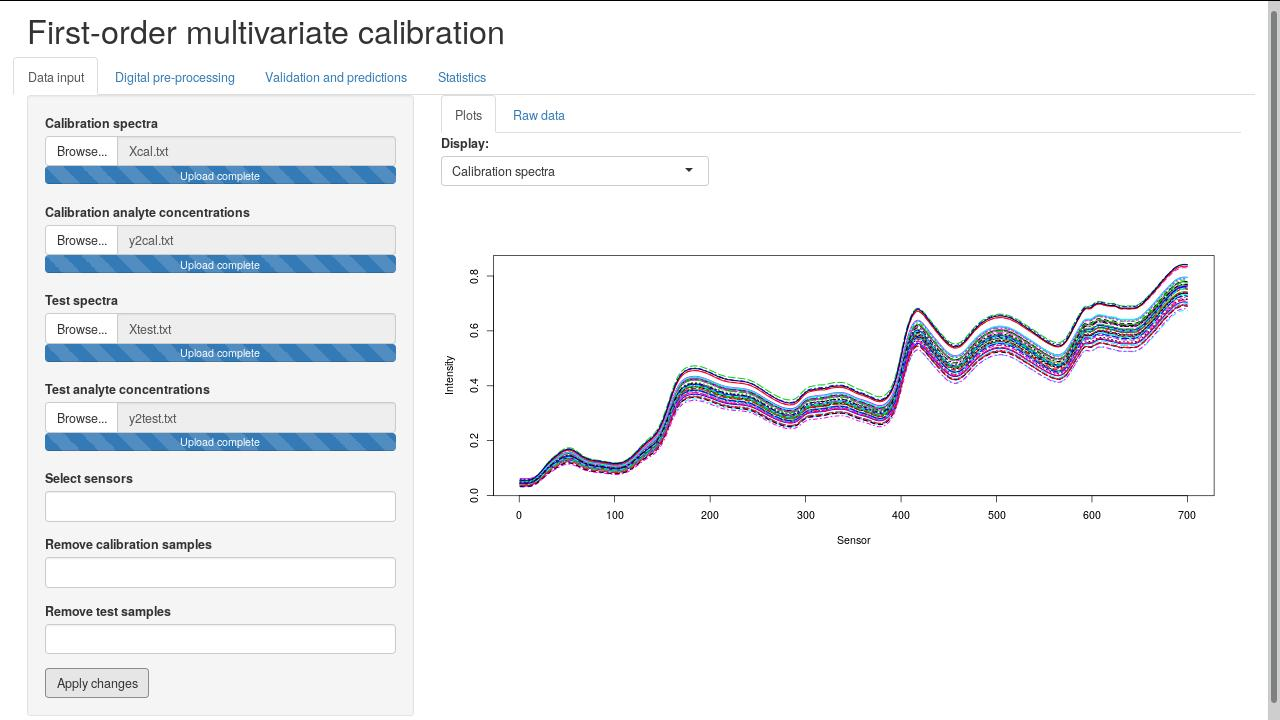
\includegraphics[width=\linewidth]{figure1.jpg}
	\caption{"Data input" tab of \texttt{MVC1\_R}, showing the browsers for
	loading the data and the calibration spectra.}
	\label{fig:1}
\end{figure}	

\section*{Student results}

\textbf{Description of the data set}

The CORN data can be freely downloaded from
\url{http://www.eigenvector.com/data/Corn}. It includes NIR spectra of a set
of 80 corn seeds and their corresponding quality parameters (moisture, protein,
fat and starch). The spectra were measured in the wavelength range 1100-2498 nm
at 2 nm intervals (700 wavelengths). The set was divided at random into a
calibration and a test set with 50 and 30 samples respectively, producing two
spectral data tables of size $700\times50$ and $700\times30$. The property
values were distributed in four tables, each of size $50\times1$ for
calibration, and four additional ones, each of size $30\times1$, for testing the
models.
\\ \\
\textbf{Data input}

To load the CORN data from the hard disk with \texttt{MVC1\_R}, students use
the tab “Data input”. Convenient browsers allow them to load the four required
files containing: (1) the matrix of calibration spectra (\texttt{Xcal.txt}),
(2) each of the vectors of calibration values for moisture, protein, fat or
starch respectively (\texttt{y1cal.txt}, \texttt{y2cal.txt}, \texttt{y3cal.txt}
or \texttt{y4cal.txt}), (3) the matrix of test spectra (\texttt{Xtest.txt}),
and (4) the corresponding test property values (\texttt{y1test.txt},
\texttt{y2test.txt}, \texttt{y3test.txt} or \texttt{y4test.txt}). Figure 1
shows the \texttt{MVC1\_R} screen for processing the oil content. Notice that
for future unknown samples, the property values are not available, in which
case the corresponding browser is not used. Clicking in "Apply ehanges"
activates plots and access to spectral and concentration values. Three
additional windows selecting spectral regions, and for removing calibration or
test samples are available. The purpose and use of these three activities is
explained in the software manual and elsewhere.\cite{olivieri18}
\begin{figure}
	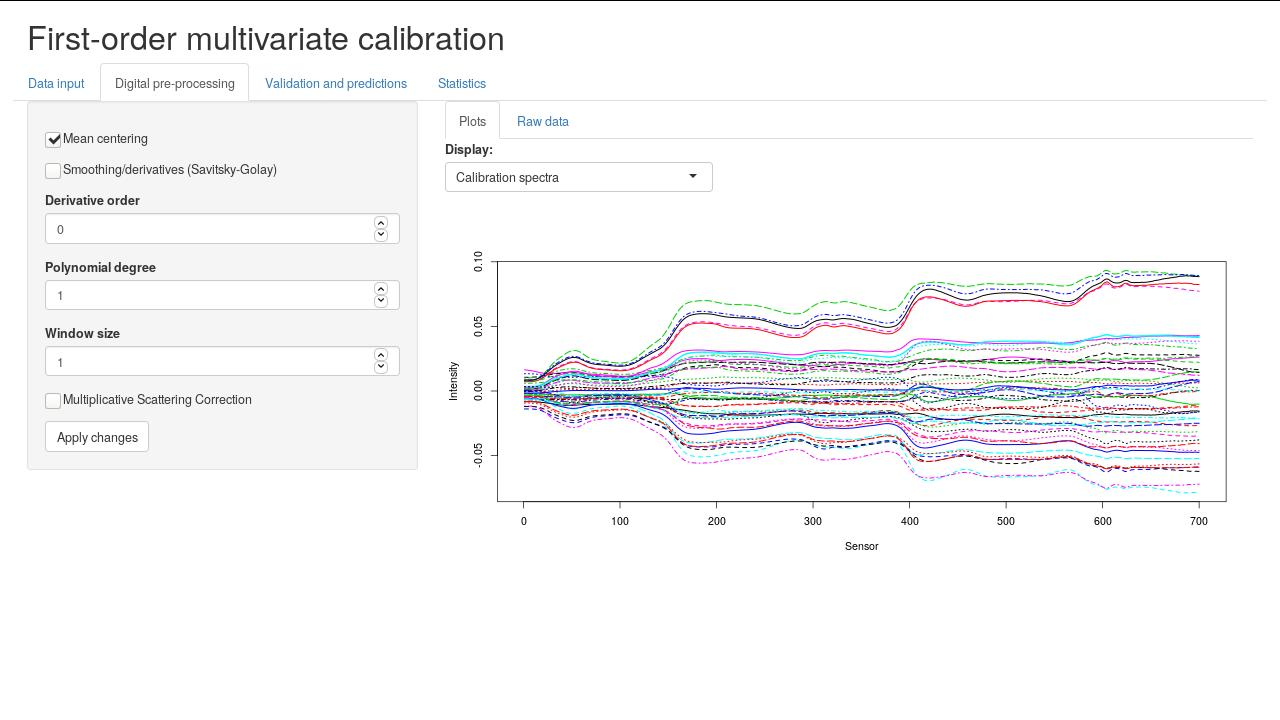
\includegraphics[width=\linewidth]{figure2.jpg}
	\caption{"Digital pre-processing" tab of \texttt{MVC1\_R}, showing the
	application of mean centering on the calibration spectra.}
	\label{fig:2}
\end{figure}
\\ \\ \\
\textbf{Digital pre-processing}

The next tab gives the possibility of digitally pre-processing the spectra
(Figure 2). Mean-centering is almost always applied and involves subtracting
from all spectra the mean calibration spectrum, and from all properties the mean
calibration value. For liquid samples, no additional activities are needed, but
solid samples usually require mathematical pre-processing in order to remove the
contribution of the NIR dispersion to the spectra, which is not related to
chemical composition. 

\begin{table*}[t]
	\centering
	\begin{tabular}{ | M{1cm} | c | M{4cm} | c | c |  }
		\hline
		Student group & Pre-processing & Optimum number of latent variables &
		RMSEP (\%) & REP (\%) \\ \hline
		1 & Mean-centering only                  & 21 & 0.040 & 1.1 \\ \hline
		2 & First derivative and mean-centering  & 14 & 0.036 & 1.0 \\ \hline
		3 & Second derivative and mean-centering &  9 & 0.045 & 1.3 \\ \hline
		4 & MSC and mean-cetering                & 19 & 0.069 & 2.0 \\ \hline
	\end{tabular}
	\caption{Students' results on the estimation of oil in the CORN data set
	using NIR-PLS analysis.}
	\label{fig:3}
\end{table*}

In \texttt{MVC1\_R}, pre-processing includes spectral derivatives and
multiplicative scattering correction (MSC). Derivatives (first or second)
remove background linear signals (first-derivative is a constant) or parabolic
ones (second-derivative is a constant). MSC removes effects which are
proportional to the mean spectrum, as is often the case with dispersion
signals.  Further information can be found in the literature.\cite{olivieri18}
In any case, after checking a digital pre-processing box, clicking in “Apply
changes” refreshes the page and updates the spectra.

To compare the effect of different pre-processing methods, students were
divided into four groups, each applying a specific method before model building
and prediction.
\\ \\
\textbf{Calibration and prediction}

Building a PLS calibration model requires to set the optimum number of latent
variables. \cite{olivieri18} These are an abstract combination of spectra
(loadings), and relative component concentrations (scores), which are needed to
represent the raw data by compression into a few variables, called
latent.\cite{olivieri18} This is usually done using a procedure called
cross-validation, as described elsewhere, \cite{olivieri18} and implemented in
\texttt{MVC1\_R} in the “Calibration and prediction” tab (Figure 3). For
cross-validation, after setting a maximum number of latent variables to be
probed (suggestion: half the number of training samples) and clicking “CV”, the
optimum value is displayed, as well as a plot of the cross-validation sum of
square errors as a function of the number of latent variables and the
corresponding statistics (see Supporting Information). The second step is to
set the number of latent variables for prediction and click in “Predict”, which
will show the estimated property values in the test samples (Figure 3).
\begin{figure}
	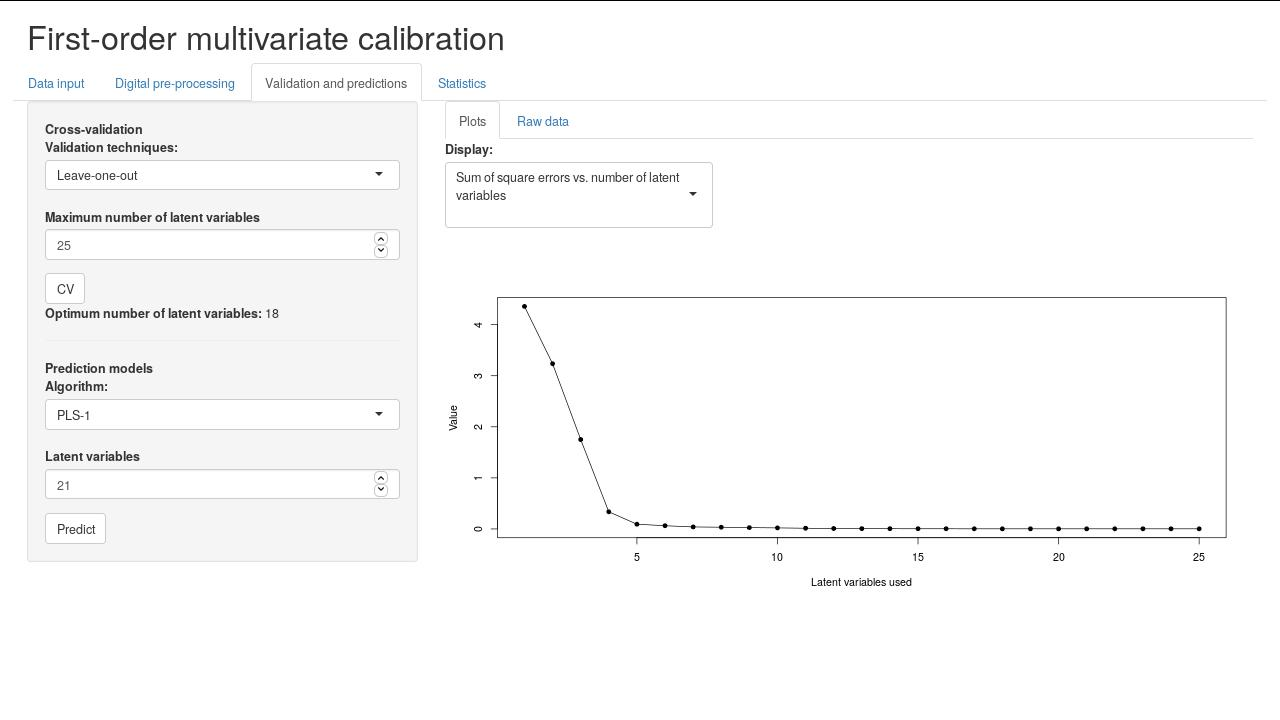
\includegraphics[width=\linewidth]{figure3.jpg}
	\caption{"Calibration and prediction" tab of \texttt{MVC1\_R}, showing the
	cross-validation results.}
	\label{fig:3}
\end{figure}
\\ \\
\textbf{Statistics}

Finally, the “Statistics” tab is useful when the reference values for the test
properties are available (Figure 4). It shows a measure of the average
prediction error, called root mean square error of prediction (RMSEP) in
concentration or property units, and the relative error of prediction (REP), in
\% with respect to the mean calibration property. \\

\begin{figure}[h]
	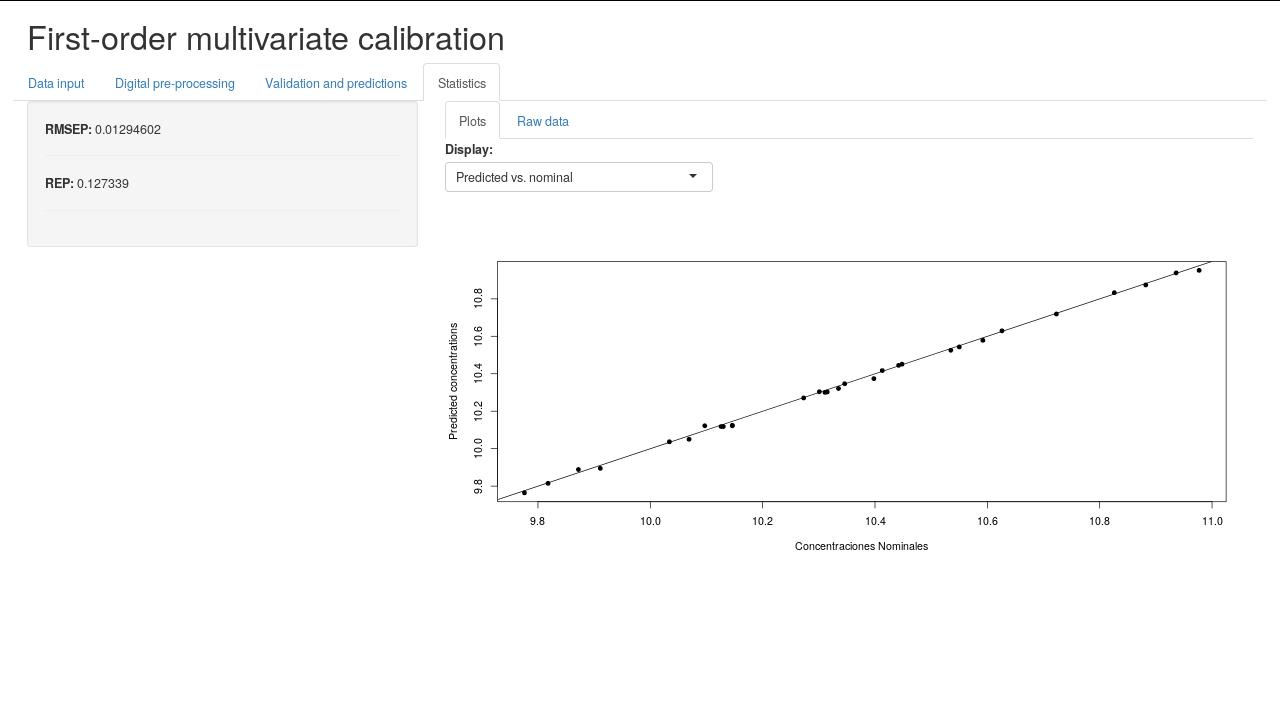
\includegraphics[width=\linewidth]{figure4.jpg}
	\caption{"Statistics" tab of \texttt{MVC1\_R}, showing the prediction errors
	and the plot of predicted vs. nominal values.}
	\label{fig:4}
\end{figure}

The specific results for oil, probably the most important oilseed quality
parameter, are shown in Table 1. Each student group applied a different digital
pre-processing, and thus they differed in the optimum number of latent variables
and average prediction error. The results triggered interesting discussions on
which pre-processing activity should be preferred. Some students argued, based
on its lowest prediction error, that first-derivative is the best pre-processing
(Table 1). Others recalled what they learned in the theoretical sessions, and
argued that, if errors are not too large, lesser latent variables are preferable
because they lead to simpler models. This is the case with the second-derivative
(Table 1). An even more interesting debate followed: is the REP for
first-derivative (1.0\%) really smaller, in statistical terms, than the REP for
second-derivative (1.3\%)? Students are asked to search the literature for
performing such a comparison, finding various tests, all of them suggesting that
the difference is not significant, and thus that second-derivative
pre-processing is to be preferred.

\newpage

\section*{Conclusions}
Practical aspects of multivariate calibration based on near infrared
spectroscopy can be conveniently learned using free online software for partial
least-squares analysis. An R Shiny application was developed for this purpose
and successfully adapted to a short chemometrics course for advanced
undergraduate chemistry students.

\section*{Associated content}
Software manual with user instructions.
This material is available via the Internet at \url{http://pubs.acs.org}.

\section*{Author information}
The authors declare no competing financial interest.

\section*{Acknowledgements}
Universidad Nacional de Rosario (Project 19B/487), CONICET and ANPCyT (Project
PICT-2016-1122) are gratefully acknowledged for financial support. TMA thanks
Instituto Polit\'ecnico Superior Gral. San Martín for an internship at
IQUIR-CONICET.

\newpage
\bibliography{references}
\bibliographystyle{ieeetr}

\end{document}
